\section{Fase di Progettazione}
    Il contenuto è stato progettato in modo statico in XHTML 1.0 Strict, la presentazione in CSS3 e il comportamento è gestito in modo dinamico con PHP7 e JavaScript, per garantire la separazione tra contenuto, presentazione e comportamento. \\
    E’ stato scelto di non progettare il contenuto in HTML5 per il fatto che HTML5 non ha raggiunto la piena compatibilità con i browser attualmente in circolazione. Tuttavia la pagina "Contatti" è in HTML5 a causa della presenza della mappa ma rispetta comunque le regole dello standard XHTML.

    \subsection{Struttura del Sito}
    La struttura della gerarchia del sito è suddivisa in pagine, alcune delle quali hanno delle sottopagine:
    \begin{itemize}
        \item Home;
        \item Auto a noleggio;
        \item Auto in vendita;
        \item Contatti;
        \item Pagina di Login;
        \item Pagina di Registrazione;
        \item Area privata (utente generico):
            \begin{itemize}
                \item Area personale;
                \item Dati Personali;
                \item Preventivi;
                \item Noleggi;
                \item Messaggi.
            \end{itemize}
        \item Area privata (utente amministratore):
            \begin{itemize}
            	\item Home amministratore;
                 \item Messaggi;
                 \item Veicoli a noleggio;
                 \item Veicoli in vendita;
                 \item Prenotazione veicoli.
            \end{itemize}
    \end{itemize}

    \subsection{Database}
    Viene riportata la rappresentazione del database, realizzata in fase di progettazione, durante la quale si è discussa la necessità di avere le diverse tabelle e per ogni tabella i necessari attributi, per poi utilizzarli al meglio.
    \begin{figure}[H]
        \centering
        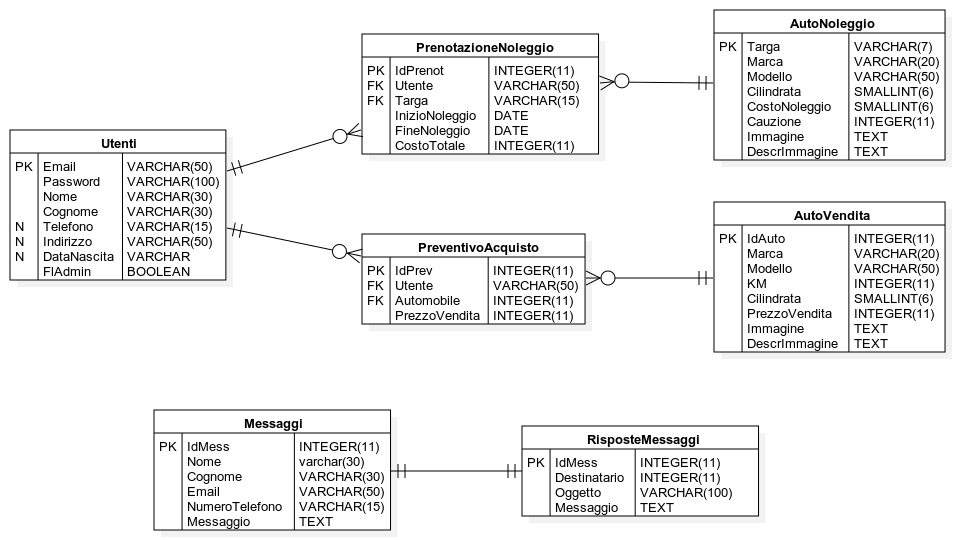
\includegraphics[width=14cm]{./img/database.png}
        \caption{Schema del database}  \label{fig:xray}
    \end{figure}
    Il database è composto dalle seguenti tabelle:
    \begin{itemize}
        \item \textbf{Utenti:} contiene i dati e le credenziali degli utenti registrati, la password è stata codificata con la funzione \textit{password\_hash} di PHP;
        \item \textbf{Messaggi:} contiene i messaggi inviati dagli utenti;
        \item \textbf{RisposteMessaggi:} contiene le risposte dell'amministratore ai messaggi inviati dagli utenti;
        \item \textbf{AutoVendita:} contiene le auto in vendita;
        \item \textbf{AutoNoleggio:} contiene le auto a noleggio;
        \item \textbf{PreventivoAcquisto:} contiene i preventivi degli acquisti delle auto effettuati dagli utenti;
        \item \textbf{PrenotazioneNoleggio:} contiene i noleggi delle auto effettuati dagli utenti;
    \end{itemize}

    Le tabelle "Messaggi" e "RisposteMessaggi" non sono in relazione con la tabella "Utenti" in quando un utente non registrato potrebbe voler mandare messaggi all'amministratore.
    
    \subsection{Accessibilità}
    Per garantire l'accesso al sito al maggior numero di categorie di utenti possibile sono stati adottati molti accorgimenti. Di seguito l'elenco dei più importanti:
    \begin{itemize}
        \item l'inserimento dei breadcrumb, che indicano sempre all'utente la posizione del sito in cui si trova;
        \item tutti i form sono provvisti di una legenda e sono stati inseriti i tag label per una migliore interpretazione dei singoli campi;
        \item l'inserimento dell'attributo alt in tutte le immagini, che rende disponibile un testo alternativo nel caso in cui l’immagine non venga caricata o l'utente non sia in grado di vederla. Per le immagini dei nuovi veicoli, la descrizione è inserita nel momento in cui viene registrato tale veicolo ed è un dato obbligatorio per completare la registrazione;
        \item l'inserimento dei link per saltare l'header e il menù di navigazione: nascosti di default, ma visibili agli screen reader. Sono posti come primi link della pagina e consentono di accedere direttamente al contenuto della pagina;
        \item l'inserimento del pulsante "TOP", sotto forma di bottone sempre visibile, che si trova a lato del content: se cliccato, ti porta all’inizio del contenuto, utile per evitare lo scroll e velocizzare la navigazione;
        \item la scelta di colori ad elevato contrasto, almeno livello AA dello standard WCAG 2.1, verificato attraverso un apposito software.
    \end{itemize}
\pagebreak